%!TEX encoding=UTF-8 Unicode

\documentclass[10pt, conference, compsocconf,pdftex,dvipsnames]{IEEEtran}

%=========================encodage fontes et langue=============================

\usepackage[utf8]{inputenc}
\usepackage[english]{babel}
\usepackage[T1]{fontenc}    % (pour les accents)

%===============================================================================

%========================= Todo notes  =========================================


%\usepackage[obeyDraft]{todonotes}
\usepackage{todonotes}
\newcommand{\mytodo}[1]{\todo[inline]{#1}}
%===============================================================================

%========================= gestion des hyperliens ==============================

\usepackage{algpseudocode}
\usepackage{algorithm}
\renewcommand{\algorithmiccomment}[1]{\State $\triangleright$ #1}
\usepackage{cite}
\usepackage{url}
\usepackage{hyperref}
\hypersetup{
    breaklinks=true, %permet le retour à la ligne dans les liens trop longs
    urlcolor= blue, %couleur des hyperliens
    linkcolor= black, %couleur des liens internes
bookmarksopen=true} 

%===============================================================================

%=========================Mathématiques========================================

\usepackage[cmex10]{amsmath} 
\usepackage{array} % tableaux pour les matrices

\newcolumntype{C}[1]{>{\centering\let\newline\\\arraybackslash\hspace{0pt}}m{#1}}

%===============================================================================

%==========================inclusion d'images===================================

%\usepackage[pdftex]{graphicx} % \includegraphics
\usepackage{caption}
\graphicspath{{./img/}}
\makeatletter
\let\MYcaption\@makecaption
\makeatother
\usepackage[font=footnotesize]{subcaption}

\makeatletter
\let\@makecaption\MYcaption
\makeatother
\usepackage{dblfloatfix}

\usepackage{epstopdf}

%==============================================================================

%==========================listes et mise en page==============================

%\usepackage{paralist} % listes : enumerate, itemize
%\frenchbsetup{StandardLists=true} %pour avoir des listes avec des points

%\usepackage[usenames,dvipsnames]{color} %de la couleur

%\usepackage{appendix} %Annexes

%==============================================================================

%=========================déclaration de titre=================================

\author{\IEEEauthorblockN{David Beniamine, Guillaume Huard}
    \IEEEauthorblockA{
        Université Joseph Fourier\\
        Laboratoire d'Informatique de Grenoble - Inria\\
        38330 Montbonnot St Martin, France\\
    david.beniamine@imag.fr, guillaume.huard@imag.fr}
}

\title{Impact of communications on XKAAPI heterogeneous applications
scheduling}
%\title{Study of communications times' impact on heterogeneous
%applications scheduling using XKAAPI }

%==============================================================================

\begin{document}

%==========================page de présentation================================


\maketitle%affichage du titre
\begin{abstract}
    High Performance Computing machines use more and more Graphical Processing
    Units as they are very efficient for homogeneous computation such as
    matrix operations. However, before using these accelerators, one has to
    transfer data from the processor to them, which can be slow. 

    To study the impact of these communications, we  provide two offline
    scheduling algorithms implementations: HEFT and convex clusters.  We
    compare them with an online scheduler on fine grain heterogeneous
    applications running on a machine with eight GPUs. Moreover, we  discuss
    the impact of unpredicted events (such as contention) on these
    algorithms, and we the limits of XKAAPI's performance model.

    Finally, our study shows that, by combining a clustering algorithm and a
    classical scheduling heuristic, we can obtain a substantial gain on the
    makespan of fine grain applications. However these results can still be
    improved as XKAAPI's performance model does not manage contention effect,
    which biased our algorithms.
\end{abstract}

\begin{IEEEkeywords}
    GPU; Clustering; Scheduling; XKAAPI; Communications;

\end{IEEEkeywords}



%==============================================================================

%=========================début réel du document===============================
\section{Introduction}

To obtain portable performances, some runtimes such as XKAAPI
\cite{gautierxkaapi} or StarPU \cite{augonnet2011starpu} allow the programmer
to describe an application as a set of tasks and dependencies.  They often use
a workstealing algorithm \cite{blumofe1995cilk} to schedule theses tasks on
the available resources. As it provide a good load balancing, this algorithm
is quite efficient on homogeneous machines. 

However nowadays, HPC computers includes many GPUs which embed their own
memory, therefore we need, we need to transfer some data from the main memory
to them. These communications must be taken into account when we try to write
efficient code on a GPU.  Indeed some work \cite{venkatasubramanian2009tuned}
have shown that their impact is such important that it can be more efficient
to recompute the same results several times to reduce the number of CPU-GPU
communications.  

Hence the basic workstealing algorithm which does not manage these
communications can suffer from bad performances on heterogeneous machines. 

\subsection{List scheduling algorithms}

The workstealing algorithm is a distributed adaptation of the list scheduling
which provide a makespan $\omega\leq2\omega^*$ where $\omega^*$ is the optimal
makespan \cite{GrahamRL1966Bounds, GrahamRL1969Bounds}. However this bound is
true for homogeneous processors and with no communications. In a model with
heterogenous machines and no communications, this bounds grows to
$\omega\leq\min(s+2-\frac{2s+1}{n},\frac{n+1}{2})\omega^*$ where $s$ is the
number of different resources and $n$ the number of processors. Hence it
does not scale for current HPC computers. 

Earliest Task First\cite{hwang1989scheduling} is an adaptation for a finite
number of identical processors with a fixed communication cost between each
couples of processors and without contention. While some tasks are not
scheduled, the algorithm try to map the earliest task that can be executed on
the processor which minimize it starting time. This algorithm provide a bound
of $\omega\leq(2+c)\omega^*$ where $c$ is the maximum cost of one
communication.  

Heterogeneous Earliest Finish Time \cite{topcuoglu2002performance}  is a two
steps algorithm: first it sort all tasks by non increasing upward rank. This
rank depends for a task $t$ of its outgoing communications and the execution
times of the tasks depending on $t$. Then it assign each task to the processor
which minimizes its completion time. This algorithm is not exactly a list
algorithm as it allows a processor to remain idle while a task is ready to be
executed.  Therefore it does not provide any bound on the execution time.
Moreover recent work \cite{Kedad-SidhoumMonnaMounieEtAl2013} have shown that
the worst case makespan can be larger than $\frac{m}{2}\omega^*$ where
$m$ is the number of tasks. Despite this result, the HEFT algorithm is widely
used (by StarPU and XKAAPI amongst others), and give some good results in
practice \cite{ferreiralima:hal-00735470}. Nevertheless, the same study have
shown that in some cases this algorithm gives better results when only the
half of the available GPUs are used.

While most of these algorithms are designed offline, they are often
implemented online in the runtimes scheduler. These online adaptations have a
lower cost than the original heuristics, however they rely on less
informations, for example HEFT online adaptation neglect the outgoing work of
a task when it compute its schedule. Therefore the offline version should be
more efficient for fine grain (ratio computations over communications)
applications as the communications can not always be overlapped with
computations.

As these algorithms are known to have better results with coarse grain
applications, it might be interesting to increase the grain of a DAG by
grouping tasks into cluster before running them.

\subsection{Clustering Algorithms}

Clustering algorithms are designed for an unbounded number of processors, they
consider the structure of the DAG and group tasks into clusters. All the tasks
which belong to one cluster are assigned to the same processor. Hence they are
executed sequentially but there are no communications between them.  

One of the most known clustering heuristic is the Dominant Sequence
Clustering\cite{yang1994dsc}, it assigns to each task a priority corresponding
to the sum of the longest path from a root node to this task and the longest
path from this task to a sink node. Then the algorithm sort the tasks by
decreasing priority and try to affect each task to the cluster which minimize
its start time among the cluster containing its predecessors. If a task can
start earlier by assigning it to a new cluster instead of an existing one, it
create a new cluster for this task. This heuristic can be very efficient as it
try to reduce the longest path through the DAG. However the graph induced by
the clusters can contain some cycles, hence it can not be directly implemented
on a middleware such as XKAAPI.

\begin{figure}[htb]
    \centering
    \includegraphics[width=0.33\textwidth]{CLANS.png}
    \caption{Different type of CLANS.}
    \label{fig:clans}
\end{figure}

The idea of CLANS
\cite{aubum1990efficient,mccreary1993partitioning,mccreary1993graph} is to
decompose the DAG into a tree of clans representing a recursive expression of
the relationship between tasks. 
%For a graph $G=(V,E)$, a set of nodes
%$X\subset V$ is a clan of the graph $G$ if and only if $\forall (x,y) \in X,
%\forall z \in V-X$, $z$ is an ancestor (or successor) of $x$ if and only if
%$z$ an ancestor (resp. successor) of $y$. 
There are three types of clans:
Independent, linear and primitive (see figure \ref{fig:clans}). Once the tree
is computed, the algorithm traverse the tree bottom up using the communication
and execution times to determine if two clans need to be merged or not.

A theoretical comparison\cite{khan1994comparison} between the algorithms DSC,
MCP (Modified Critical Path, similar to DSC), MH, HU (lists algorithms) and
CLANS have shown that CLANS is robust and efficient for a large and diverse
set of graphs. All the others algorithms give very bad performances for graphs
with a fine grain. However this algorithm is very complex as we need to
extract the tree of clans, and as DSC it can produce a cluster graph with
cyclic dependencies. Hence it is not suited for our problem. 

\begin{figure}[htb]
    \centering
    \includegraphics[width=0.31\textwidth]{conv.png}
    \caption{Convex and non convex group of tasks.}
    \label{fig:conv}
\end{figure}


The convex clustering algorithm\cite{lepere2002new} produces an acyclic graph
of clusters.  Indeed a cluster $C$ is convex if and only if $\forall\ (x,z)\
\in\ C$ all task $y$, such that $x\ \prec\ y\ \prec\ z$, is in $C$ (see
figure \ref{fig:conv}). By this property, we know that there are no two way
communications between two clusters. Moreover as the graph obtained by merging
the tasks inside a cluster is a Direct Acyclic Graph, it allow us to run
any scheduling algorithm on it.

\subsection{Key Issues}

Although the GPUs are able to reduce substantially the execution time of some
tasks, we need to transfer data from the main memory to them before the
execution. Previous work\cite{ferreiralima:hal-00735470} have shown that it is
possible to reduce the impact of these communications costs by overlapping
them with computations and by using sophisticated scheduling algorithms such as
HEFT.  However, this work have also highlighted the fact that some contention
can occur on machines with many GPUs linked to the processors by an
interconnection network.

In this study, we use machines with one or several GPUs, and we aim at showing
and measuring the impact of the communication times on the scheduling of HPC
applications. All the list algorithms cited before are efficient for coarse
grain applications however when the grain is fine enough, as they do not
consider the whole structure of the DAG. Therefore our analysis focus on very
fine grain applications. 


\mytodo{Modify percentage after expe}
To reach that goal, we provide the implementation of  a static scheduler and
several heuristics within the parallel runtime XKAAPI. Our experimental study
shows that by combining list heuristics and clustering algorithms, we can
reduce the impact of communications times. Indeed the offline version of HEFT
can give a gain of $59\%$ compared to the makespan of the online one when the
volume of communications is large enough.  Moreover, using a clustering
algorithm before HEFT, we can reduce the makespan of one scheduling up to
$64\%$ compared to the online HEFT.

First we present our implementation of the convex cluster algorithm in
XKAAPI's runtime, and our adaptations  in section \ref{sec:impl}. Then we use
this scheduler to analyse the impact of communication in section
\ref{sec:exp}. And finally we give our conclusions and some future work on
section \ref{sec:cncl}.

\section{Implementation of an offline scheduler in XKAAPI's runtime}
\label{sec:impl}

By default, XKAAPI uses an online scheduler and compute data dependencies in a
lazy way. Its scheduler provides various heuristics, among them, we can find
an online adaptation of the HEFT algorithm. The main difference between this
version and the original one is that the first one cannot sort the ready tasks
according to the upward rank as the DAG is not fully known.  Still the online
heuristic works with actual time when the offline one uses predicted times thus
only the first one is able to adapt to unexpected effects such as contention.

\subsection{XKAAPI scheduler and performance model}
\label{sec:impl-kaapi}

XKAAPI provides an API for writing scheduling heuristics designed for online
algorithms. One can write three callbacks methods. The first (\texttt{init})
is launched during the initialization of the runtime before the execution of
the program.  The second one (\texttt{push}) is called each time a tasks is
ready to be executed and must return the processor on which the tasks should
be run. As XKAAPI is a workstealing runtime, a task is always executed as soon
as all its dependencies are satisfied and a processor is ready to run it. The
last one (\texttt{steal}) is executed when a processor wants to steal a task
from another and must return the task to be stolen.

Although this API is minimalistic, we can extract the DAG from the ready tasks
list when the middleware calls the \texttt{init} callback. Therefore we are
able to run an offline scheduler during this phase and apply its decisions in
the \texttt{push} and \texttt{steal} functions.  However this functions only
choose the processor on which a task is executed. As XKAAPI tries to execute
each task as soon as possible, to set the execution order of the task which
belong to the same processor, we need to add some internal (empty)
synchronization tasks.

XKAAPI also contains a performance model which provides for each task, a
prediction of its execution time on a each processor. This model can also
estimate the time needed to transfer $n$ bytes of data from one processor to
an other. This predictions are derived from the traces of one (or several)
previous calibration runs. We will discuss the impact of these calibration
runs an how this model can be biased in section \ref{sec:exp}. It is important
to notice that even the online adaptation of HEFT uses this performance model.

\subsection{Offline scheduling}
\label{sec:impl-off}
By default, in XKAAPI, each processor has a part of the work in his queue of
tasks, nevertheless it is able to maintain a centralized list of ready tasks.
As each task has a pointer to all its successors, the dependencies graph is
known within the runtime. However as the convex cluster algorithm need to
compute ancestors and descendants of every nodes of the DAG, with this pointer
based representation, computing these relationships can be costly. Therefore
the first step of our static scheduler is to extract the DAG into an adjacency
matrix and to run a Warshall Algorithm which compute all the parenthood
relations. This algorithm has a worst case in $O(|V|^3)$ where $|V|$ is the
number of nodes of the DAG, and a mean case in $O(|V|^2)$.

\begin{algorithm}[h!]
    \centering
    \caption{Convex cluster}
    \label{algo:conv-clust}
    \begin{algorithmic}[1]
        \Function{Extract\_clusters}{Graph $G=(V,E)$}
        \State $Part \gets NULL$
        \State $CurMax \gets 0$
        \For{$rdt \in  [0 .. MaxRandomTry ]$ }\label{algop:main-loop}
        \State $pivot \gets RandomNode(G)$
        \State
        $<A,A^{\sim},A^<,A^>> \gets Decompose4(G,pivot)$\label{algop:init-part}
        \Comment Decompose G into four partitions 
        \Comment $pivot$, nodes independent from $pivot$, 
        \Comment $pivot$'s ancestors and $pivot$'s successors fig
        \ref{fig:conv-decomp1} 
        %, \textbf{Cost: $O(|V|)$}
        \\
        \State $Update\_partitions(<A,A^{\sim},A^<,A^>>)$
        \label{algop:update-part}
        \Comment $A^<$ and $A^>$ becomes predecessors 
        \Comment (resp. successors) of all nodes  
        \Comment from $A$ and $A^{\sim}$, fig 
        \ref{fig:conv-decomp2}
        \\
        %        \Comment \textbf{Cost:$(|A^<| + |A^>| )*|A^{\sim}| = O(|V|^2)$}
        \If{$MAX(|A|,|A^{\sim}|) > CurMax$} \label{algop:part-choice}
        \\
        %\Comment We have found a better decomposition
        \State $CurMax \gets MAX(|A|,|A^{\sim}|)$
        \State $Part \gets <A,A^{\sim},A^<,A^>>$
        \EndIf
        \EndFor
        \ForAll{$p \in Part$}
        \If{$|p| > MaxClusterSize$}\label{algop:rec-stop}
        \State $Extract\_Clusters(p)$
        \Comment Divide the partition if large enough
        \Else
        \State $Add\_Cluster(p)$
        \Comment Save the cluster
        \EndIf
        \EndFor
        \EndFunction
    \end{algorithmic}
\end{algorithm}

\begin{figure*}[t!]
    \centering
    \begin{subfigure}{0.22\textwidth}
        \centering
        \includegraphics[width=0.7\textwidth]{conv-decomp0.png}
        \caption{Original graph.}
        \label{fig:conv-decomp0}
    \end{subfigure}
    ~
    \begin{subfigure}{0.25\textwidth}
        \centering
        \includegraphics[width=0.7\textwidth]{conv-decomp.png}
        \caption{\texttt{Decompose4()}}
        \label{fig:conv-decomp1}
    \end{subfigure}
    ~
    \begin{subfigure}{0.25\textwidth}
        \centering
        \includegraphics[width=0.7\textwidth]{conv-decomp2.png}
        \caption{\texttt{Update\_Partitions()}}
        \label{fig:conv-decomp2}
    \end{subfigure}
    \caption{Decomposition and update step of convex cluster algorithm.}
    \label{fig:conv-decomp}
\end{figure*}


Once these dependencies are computed, we are able to run our implementation of
the convex cluster algorithm (see algorithm \ref{algo:conv-clust}). The
original convex cluster algorithm select two independent random nodes and uses
them to divide the group into four partitions $A$ and $A^{\sim}$ which are
independent, their predecessors $A^<$ and successors $A^>$. Once these
partitions are computed, either the smallest of $A$ and $A^{\sim}$ is large
enough and all the partition are recursively divided, or they are all grouped
into one cluster. 

Our implementation is close to this algorithm however as it is designed for a
theoretical machine with an unbounded number of identical processors, it
requires a few adjustments, for example in the original version the recursion
stops when the partition size is less than twice the communication cost. As we
do not have a unitary communication cost, the maximal size for a cluster is
given as a parameter and the recursion stops when a cluster is smaller than
this size (see line \ref{algop:rec-stop}). 
%Then, the clusters are mapped on the processors using the HEFT algorithm. 

\begin{figure}[htb]
    %        \begin{subfigure}{0.5\textwidth}
    %        %    \hspace{-20pt}
    %            \scalebox{0.6}{
    %                \input{img/rdtry_m1100_b100_maxDePartMin.tex}
    %            }
    %            \caption{Original heuristic.}
    %            \label{fig:RdtMaxDeMin}
    %        \end{subfigure}
    %   \hspace{-15pt}
    %        \begin{subfigure}{0.5\textwidth}
    \scalebox{0.65}{
        \centering
        \input{img/rdtry_m1100_b100_maxDePartMax.tex}
    }
    %            \caption{Our heuristic.}
    %            \label{fig:RdtMaxDeMax}
    %        \end{subfigure}


    \caption{Heuristic used to choose the best clustering, on       
    a Cholesky reduction, on Mapuche.}
    \label{fig:Rdt}
\end{figure}

In addition, the original algorithms kept the cluster where the smallest
partition was the larger and recursively divide either all the partition or
none of them. These criteria gave unstable results. Hence we always keep the
clustering giving the largest cluster (see line \ref{algop:part-choice}) and
we choose to recursively divide each individual clusters if it is large enough
(line \ref{algop:rec-stop}). We can see in figure \ref{fig:Rdt} that with this
heuristic, the algorithm stabilize quicker than in with the original one.
Moreover if we do not reach the best result obtained by the original
algorithm, when the stabilisation occurs, we provide a better schedule with
our heuristic.

The two important (and costly) steps of this algorithm are the initial
decomposition into four clusters, and their update to keep the clusters
balanced.  Starting from the graph shown on figure \ref{fig:conv-decomp0}, we
choose randomly a pivot (the node $7$) and we put all the others nodes in one
of the three groups its predecessors $A^<$, its successors $A^>$ all the
others $A^{\sim}$. At the end of this step we have the clustering displayed on
figure \ref{fig:conv-decomp1}. As we can know the relationship between two
nodes in constant time from the precomputed matrix .This step costs only
$O(|V|)$ comparisons. During the second step, we compare each nodes of $A^<$
and $A^>$ with the nodes of $A^{\sim}$ to determine the common predecessor
(resp successors) of $A$ and $A^{\sim}$ keep their initial placement, the
others are moved in the group $A$.  This way, we obtain the clustering
presented on figure \ref{fig:conv-decomp2}. The second step has a cost of:
$$C=(|A^>|+|A^<|)*|A^{\sim}|$$ 
we know that at the end of the first step $|A|=1$ which implies: 
$$|A^>|+|A^<|+|A^{\sim}|=|V|-1$$
thus:
$$C=(|V|-1-|A^{\sim}|)*|A^{\sim}|$$ 
The two terms are bounded by $|V|$ so we have: 
$$C\leq|V|^2$$
%and so if $|A^{\sim}|=\frac{|V|}{2}$,
%$$C=(|V|-1-\frac{|V|}{2})*\frac{|V|}{2}=\left(\frac{|V|}{2}\right)^2-\frac{|V|}{2}$$
%hence we have: 
hence :
$$C=O(|V^2|)$$ 
Finally, if we assume that the clusters are balanced it takes
$log\left(\frac{|V|}{MaxClusterSize}\right)$ calls to stop the recursion, as
the two first step are repeated $MaxRandomTry$ times, the
cost of our implementation is:
$$O\left(MaxRandomTry*|V|^2*log\left(\frac{|V|}{MaxClusterSize}\right)\right)$$

As the clustering phase aims at increasing the grain of the graph, we need to
be sure that each cluster will behave as one single task. Therefore in the
runtime, we have to add some empty synchronization tasks at the beginning and
at the end of each clusters as shown in figure \ref{fig:conv-int} (white
diamond shaped nodes). Indeed with the clusters of the figure
\ref{fig:conv-decomp2}, without these tasks,  as XKAAPI uses a work stealing
algorithm to execute a task as soon as it is ready, if the clusters $A^<$ and
$A^{\sim}$ are executed on the same processor, the second one might start
before the end of the first, delaying the execution of the cluster $A$.
Although these synchronization tasks increase the size of the graph, they are
empty, and as the cost of a task is very low in XKAAPI, the overhead induced
is negligible. Once the DAG of clusters has been computed, we can find the
mapping between the clusters and the processors according to the HEFT
algorithm for instance. 

\begin{figure}[t!]
    \centering
    \begin{subfigure}{0.24\textwidth}
        \centering
        \includegraphics[width=0.7\textwidth]{conv-internal.png}
        \caption{Graph after adding the internal tasks.}
        \label{fig:conv-int}
    \end{subfigure}
    ~
    \begin{subfigure}{0.1\textwidth}
        \centering
        \includegraphics[width=\textwidth]{conv-clust.png}
        \caption{Cluster graph.}
        \label{fig:conv-clust}
    \end{subfigure}
    \caption{Final transformations from a graph of tasks to a graph of
    clusters.}
    \label{fig:conv-end}
\end{figure}

These two steps have a cost $\leq |V|^2$ hence our offline scheduler has a
theoretical worst case cost in $O(|V|^3)$ due to the Warshall algorithm,
however the mean case cost is still $O(log(|V|)*|V|^2*MaxRandomTry)$ (due to
the convex cluster algorithm).  Although this cost is quite high, in some
domains such as physical simulation, applications are often
iterative and regular. This means that the same parallel code has the
opportunity to be executed several times in a row using the same schedule.
Hence we can amortize that initial cost. As our aim is to study the impact of
communication times, we will not try to amortize this initial cost in the
following experiments and we will separate it from the execution times in our
results.

\section{Analysis and reduction of the communication times}
\label{sec:exp}

We use our scheduler to study the impact of communications on two different
machines which are described in section \ref{sec:exp-set}. For this
experimental analysis we compare the online HEFT with our offline implementation,
as the first one does not consider the communication times as much as the
other. Then we combine it with a clustering phase to take the communications
into account at a global scale. All these heuristics are tested on a
Cholesky decomposition as this application induced some contention on a
previous study \cite{ferreiralima:hal-00735470}.


\subsection{Experimental setup}
\label{sec:exp-set}

\begin{table*}
    \centering
    \scalebox{0.78}
    {
        \begin{tabular}{|C{1.7cm}|c|C{1.1cm}|C{1.3cm}|C{1.2cm}|C{1.2cm}|C{1.6cm}|
            C{1.3cm}|C{1.4cm}|C{1.2cm}|C{1.6cm}|C{1.4cm}|C{1.8cm}|}
            \hline
            \textbf{Name} & \textbf{\#CPU} & \textbf{\#Core / CPU} 
            &\textbf{ CPU vendor} & \textbf{CPU model}  &
            \textbf{CPU freq (Ghz)} & 
            \textbf{Memory (Gio)} & \textbf{\#GPU} & 
            \textbf{GPU vendor} & \textbf{GPU model} &  
            \textbf{GPU memory}&\textbf{GPU clock freq (Ghz)} 
            &\textbf{ CUDA capability} \\
            \hline
            Mapuche & 1 & 4 & Intel & Core I7-2600 & 3.4 & 8 & 1 & Nvidia &
            NVS 300 & 512 MB DDR3& 1.23 &1.2 \\
            \hline
            IdGraf & 2 & 6 & Intel & Xeon X5650 & 2.67 & 72& 8 & Nvidia &
            Tesla C2050 & 3GB GDDR5 & 1.15 & 2.0 \\
            \hline
        \end{tabular}
    }
    \caption{Hardware used for the experiments.}
    \label{table:machines}
\end{table*}

All the experiment presented in this study, including those presented in the
previous sections, have been run on one or the other
of the two following machines:
Idgraf\footnote{\url{http://digitalis.inria.fr/index.php/Usage\#idgraf}} a HPC
workstation with 12 cores and 8 GPUs managed by Grid5000 and Mapuche a
personal workstation with 4 CPUs and one GPU. The hardware of these machines
is described more precisely in table \ref{table:machines}, for both machines
hyper-threading and thermal throttling are turned off. 

Idgraf runs on a Debian squeeze with a Linux kernel
3.2.0.2-amd64. Mapuche's Operating System is an Ubuntu 12.10 LTS with a
Linux kernel 3.2.0-40. 


\begin{figure}[htb]
    \centering
    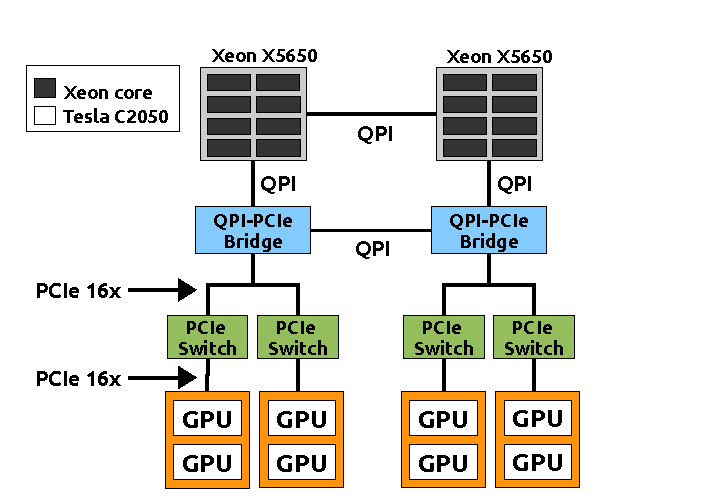
\includegraphics[width=0.48\textwidth]{idgraf-topo-2012.pdf}
    \caption{Idgraf's topology\cite{gautierxkaapi}.}
    \label{fig:idgraf}
\end{figure}

It is important to note that Idgraf has a hierarchical topology as shown in
figure \ref{fig:idgraf}, the eight GPUS are split over two PCI Bridge which
are linked together. Each bridge manage 4 GPUs separated in two groups which
belong to two different switches. With this particular topology, simultaneous
communications involving several GPUs might lead to contention on the PCie
switches, this contention will be highlighted in section
\ref{sec:exp-exp-perf}.

\mytodo{update default param}
Regarding our algorithms, unless stated otherwise, we use the following
parameters: $NbRandomTries=\sqrt{|V|}$, $MaxClusterSize=10$, and for the
studied applications $MatrixSize=1000$, $BlocSize=MatrixSize/10$ for Mapuche
and $BlocSize=MatrixSize/20$ for Idgraf.  as Idgraf has way more computational
resources then Mapuche, HEFT is efficient with a smaller grain, hence we
decrease the $BlocSize$, to reduce even more the grain of the application.

For each curve presented in the following section, each points represent the
mean runtime of $15$ to $30$ different runs with the same parameters, and a
confidence interval of $95\%$ is displayed as an error bar.

Finally, by default the execution time presented for the algorithms HEFT
offline, and convex cluster correspond to the total time minus the overhead
induced by the static scheduler.

\subsection{Comparison of online and offline heuristics}
\label{sec:exp-exp-perf}

There are two important differences between the online and the offline version
of the HEFT algorithm, the first one is that the offline algorithm sorts the
tasks by upward rank, which means that a task priority is related to the
length of the chain of tasks that depends on it. As the online version does
not have a global vision of the DAG, it maps each task to a processor as soon
as it is ready, without sorting all the ready tasks, which can result on bad
scheduling decisions.  However, the second difference is that the offline
algorithm only uses theoretical execution and communication times while the
online one uses theoretical times for predictions but takes its decisions at
runtime. Hence, if there is some contention, the online algorithm will see
that a processor which should be ready is not and will adapt its decisions.

To show these differences, compare the makespan of a Cholesky decomposition on
our two machines using all the available GPUs  with the two versions of HEFT.
The results are displayed in figure \ref{fig:OnOff}. The first important point
is that, on Mapuche (figure \ref{fig:OnOffMapuche}), the offline algorithm
provides always an equivalent or better makespan than the online one. In the
best case can observe a gain of $59\%$. This result confirms our first idea:
when we are in a configuration where there are many communications and not
enough computations to overlap them (small matrix sizes) , we can obtain a
substantial gain by using an heuristic specifically designed to minimize these
communications.

\begin{figure}[h!]
    %\begin{adjustwidth}{}{-3cm}
    \centering
    \begin{subfigure}{0.5\textwidth}
%        \hspace{-20pt}
        \scalebox{0.65}{
            \input{img/mat-size-mapuche-noInt-calibrate.tex}
        }
        \caption{Comparison on Mapuche.}
        \label{fig:OnOffMapuche}
    \end{subfigure}
%    \hspace{15pt}
    \begin{subfigure}{0.5\textwidth}
        \scalebox{0.65}{
            \input{img/mat-size-idgraf-8gpu-cal8GPU.tex}
        }
        \caption{Comparison on Idgraf.}
        \label{fig:OnOffIdgraf}
    \end{subfigure}
    %\end{adjustwidth}
    \caption{Online vs offline HEFT scheduling, on Cholesky decomposition, on both
    machines.}
    \label{fig:OnOff}
\end{figure}

Nevertheless, the same experiment on Idgraf gives a different result, indeed
we can see in figure \ref{fig:OnOffIdgraf} that if we still have a gain of
$17.7\%$ with a matrix of size $800$. However, when we increase this size, the
gap shrinks and finally, when it exceed $1400$ the online algorithm gives
better results up to $10.2\%$. As the main difference between the two machines
is the number of GPUs and as the advantage of the online scheduler compared to
the offline one is the capacity to adapt to a biased model, our first
hypothesis, is that a contention which cannot be anticipated by the model
appears on the PCI buses (see figure \ref{fig:idgraf}) when we use all the
GPUs. 

\mytodo{Change this par when new exp}
To prove this hypothesis, we run the same experiment on one, two, four
and eight GPUs with both algorithms. The figure \ref{fig:ContentionGpu} shows
the results of the both heuristics with zero to eight GPUs. We can see that we
obtain equivalent or better makespan using only one GPU rather then eight.  In
addition, we have found that for many tasks, the predicted execution times
(i.e. the execution time extracted from the calibration runs) were increasing
as we were using more GPUs. As we need a data transfer to know when a GPU task
is finished, our performance model includes a small communication in the
predicted execution times. However when we some contention appears, this
communication take more time and modify substantially the predicted execution
time which biased our algorithms.  However, we can easily avoid this bias by
performing our calibration run with only one GPU.  Doing this, we are able to
reduce the execution time of $24.7\%$ on 8 GPUs as we can see on figure
\ref{fig:ContentionTrick}. All these results validate our hypothesis, there is
some contention on the PCI buses.

\begin{figure}[htb]
    \centering
    \begin{subfigure}{0.5\textwidth}
        \scalebox{0.6}{
         %   \input{img/gpu-idgraf-c0-cal1GPU-off.tex}
            \input{img/gpu-idgraf-c0-m800.tex}
        }
        \caption{Effect of the number of GPUs used during the execution.}
        \label{fig:ContentionGpu}
    \end{subfigure}
    \begin{subfigure}{0.5\textwidth}
        \scalebox{0.6}{
            \centering
            \input{img/mat-size-idgraf-8gpu-cal1-8GPU.tex}
        }
        \caption{Effects of the number of GPUs during the calibration.}
        \label{fig:ContentionTrick}
    \end{subfigure}
    \label{fig:Contention}
    \caption{Analysis of the contention, on the execution time of a 
    Cholesky decomposition, on Idgraf.}

\end{figure}

Finally, we have clearly shown that the offline algorithm is able to give
better results (up to $59\%$ in our experiments) by avoiding some
communications. However, if the model does not fit to the reality (for example
when there is some contention), our offline algorithm is biased. Hence
we can think about implementing an hybrid scheduler which takes initial
decisions statically and adapts (or recompute them) if the actual execution
times do not match to the expected ones.

\begin{figure*}[t!]
    %\begin{adjustwidth}{}{-3cm}
    \centering
    \begin{subfigure}{0.4\textwidth}
        \hspace{-20pt}
        \scalebox{0.6}{
            \input{img/mat-size-c10-mapuche.tex}
        }
        \caption{Mapuche.}
        \label{fig:MatMapuche}
    \end{subfigure}
    \hspace{15pt}
    \begin{subfigure}{0.55\textwidth}
        \scalebox{0.6}{
            \input{img/mat-size-bm20-m600_1100-4GPU-cal1GPU-idgraf.tex}
        }
        \caption{Idgraf, $BlocSize=MatrixSize/20$.}
        \label{fig:MatIdgraf}
    \end{subfigure}
    %\end{adjustwidth}

    \caption{Square matrix dimension impact on convex cluster and HEFT
    algorithm, on a Cholesky decomposition, on both machines.}
    \label{fig:Mat}
\end{figure*}


\subsection{Analysis of the clustering algorithm}
\label{sec:exp-exp-clust}

In the following experiments, we increase the grain of the DAG using the
convex cluster algorithm before running the offline HEFT algorithm. Using this
combination, we will show that we can have an even better gain than with the
offline or the online algorithm only.

\mytodo{Update when new expe}
Our first experiment on the convex cluster algorithm aims at showing for which
matrix size this heuristic can be useful. We can see in figure
\ref{fig:MatMapuche} that as for the offline HEFT, the convex cluster
algorithm gives better results for small matrices, with a gain up to $28.5\%$
on Mapuche with a matrix size of $800*800$. In our implementation of the
convex cluster algorithm, we can set the maximum size of a cluster as a
parameter. Hence the following experiments will show the impact of this
parameter on the schedule. 

\begin{figure*}[htb]
    %\begin{adjustwidth}{}{-3cm}
    \centering
    \begin{subfigure}{0.4\textwidth}
        \hspace{-20pt}
        \scalebox{0.6}{
            \input{img/clust-size-c0-80_m1000_b100-improved-log.tex}
        }
        \caption{Mapuche.}
        \label{fig:ClustersMapuche}
    \end{subfigure}
    \hspace{15pt}
    \begin{subfigure}{0.55\textwidth}
        \scalebox{0.6}{
            %\input{img/clust-size-full-bm20-m1000-4GPU-cal1GPU-idgraf.tex}
            \input{img/mat-size-bm20-1100-8GPU-cal1GPU-idgraf.tex}
        }
        \caption{Idgraf, $BlocSize=MatrixSize/20$, $8$GPUs.}
        \label{fig:ClustersIdgraf}
    \end{subfigure}
    %\end{adjustwidth}

    \caption{Effect of the maximum size of clusters on the convex cluster
    algorithm, on a Cholesky decomposition, on both machines.}
    \label{fig:Clusters}
\end{figure*}

\mytodo{adapter le texte après exp}
\mytodo {Refaire la courbe \ref{fig:MatMapuche}}
On idgraf, to obtain a better scheduling, the convex clustering still gives a
better schedule than the online HEFT as we can see in fiugre
\ref{fig:MatIdgraf}.  The best case tested in our experiment is for a matrix
size of $600*600$ where we reduce the makespan of $64\%$.

From this experiment, it is clear that with small matrices, we can highly
improve the scheduling obtained by the online algorithm. For the next
experiments, we will use a small matrix $1000*1000$ and we will keep the same
bloc sizes as for this experiments. Their objective is to study the impact
of the maximal size of one cluster on the scheduling.

By increasing the maximum size of a cluster (see algorithm
\ref{algo:conv-clust}, line \ref{algop:rec-stop}), we increase the grain of
the graph and we reduce the amount of communications that HEFT has to manage.
However we also reduce number of possible schedules.

Figure \ref{fig:ClustersMapuche} shows the results of our last experiment on
Mapuche. We can see that we need large clusters $\geq 30$ to obtain the maximal
gain. However if we use a cluster size larger than $70$, it seems that we
loose to much scheduling freedom and the HEFT algorithm cannot give an efficient
scheduling anymore. Finally, we can notice that with $MaxClusterSize=35$ we
reduce the execution time by $48\%$ in comparison to the offline HEFT
algorithm and $59.5\%$ in comparison to the online version.

In figure \ref{fig:ClustersIdgraf}, we display the results of the
experiment on Idgraf using $8$ GPUs, we can see that the best cluster size is
quite different than for Mapuche. This difference comes from the fact that as
Idgraf embed more processors than Mapuche, hence it needs a larger graph (i.e.
smaller clusters) to use them efficiently. Still, with the convex clustering,
we can obtain a gain of $34.7\%$ on Idgraf compared to the online heft, which
correspond to a gain of $11\%$ compared to the offline one.



\section{Conclusions and future work}
\label{sec:cncl}
During this study, we have worked on
XKAAPI\cite{gautier2007kaapi,gautierxkaapi}, an existing middleware for
parallel programing in which we have implemented a static scheduler with
several heuristics. Then, we have used these heuristics to evaluate the impact
of communication times on the maskespan of fine grain applications.

\subsection{Main contributions}
\label{chap:cncl-contrib}

Our first contribution is the implementation of a static scheduler using
a classical algorithm, Heterogeneous Earliest Finish Time combined to a
clustering algorithm, convex clusters.

This study focus on fine grain applications, where the communication
times have a huge impact on the total execution time. Using an offline
algorithm, we are able to reduce the makespan of an application up to
$59\%$. Some contention effects have been highlighted on an heterogeneous
machine with 8 GPUs. 

Our study also shows some limits of the performance model used by XKAAPI
and we have proposed one technique to reduce their effects on the offline
algorithms. However to improve upon the results of offline schedulers we need a
performance model which takes contention effects into account.

\mytodo{update percentage}
Finally by increasing the grain of a DAG with the clustering algorithm before
running the offline HEFT algorithm, we observe a substantial gain up to $64\%$
on the makespan, compared to the online HEFT.

However, these results do not take into account the overhead needed to run
scheduling algorithms which is not negligible. Hence, we still need to work on
the ability to reuse a schedule to amortize its initial computation cost. 

To conclude, this study highlight the fact, that when the grain is fine
enough, and if we use heterogeneous machines, it is worthwhile to use some 
complex scheduling algorithm to reduce the impact of communication times.
However we also show that when the grain is large enough, it is more
efficient to use a simpler online scheduler.

\subsection{Future work}
\label{chap:cncl-work}

For all the experiment shown in this study we have removed the overhead of the
offline scheduler, however this overhead is not negligible. Therefore some
future work will consist on giving the ability to reuse a (partial) schedule
for iterative applications (such as physical simulation).

%Additionally, we would like to complete our study by a comparison with some
%others algorithms designed to reduce the impact of communication times such as
%DSC or CLANS. However these algorithms might create a cyclic DAG of clusters
%which is incompatible with XKAAPI's runtime. Hence we need either to adapt
%them or to run another algorithm after them to merge or cut some clusters to
%remove the cyclic dependencies.

Finally an interesting perspective would be to design an adaptive algorithm
able to update the different parameters of the heuristic tested in this study,
and which combine an initial (offline) schedule with an online tool allowed to
modify it if the actual times are not close enough to the predictions. Moreover
using such an algorithm, we could avoid the initial calibration run required
by XKAAPI's perfomance model.

\section*{Acknowledgments}

Experiments presented in this paper were carried out using the Grid'5000
experimental testbed, being developed under the INRIA ALADDIN development 
action with support from CNRS, RENATER and several Universities as well as
other funding bodies (see \url{https://www.grid5000.fr}).


We'd like to thanks Thierry Gautier for the figure \ref{fig:idgraf} extracted
from the paper XKAAPI IPDPS 2013 \cite{gautierxkaapi}.


%=========================Bibliographie========================================
%\IEEEtriggeratref{3}

\bibliographystyle{IEEEtran}
\bibliography{ConvexGpu}

\mytodo{Remove the todo list}
\listoftodos
%==============================================================================

%=========================annexes==============================================

%newpage
%\appendix{ \textbf{Annexe }}

%==============================================================================
\end{document}

